
\input{../../2021/style/preamble4tex}
% math spaces
\ifdefined\N                                                                
\renewcommand{\N}{\mathds{N}} % N, naturals
\else \newcommand{\N}{\mathds{N}} \fi 
\newcommand{\Z}{\mathds{Z}} % Z, integers
\newcommand{\Q}{\mathds{Q}} % Q, rationals
\newcommand{\R}{\mathds{R}} % R, reals
\ifdefined\C 
  \renewcommand{\C}{\mathds{C}} % C, complex
\else \newcommand{\C}{\mathds{C}} \fi
\newcommand{\continuous}{\mathcal{C}} % C, space of continuous functions
\newcommand{\M}{\mathcal{M}} % machine numbers
\newcommand{\epsm}{\epsilon_m} % maximum error

% counting / finite sets
\newcommand{\setzo}{\{0, 1\}} % set 0, 1
\newcommand{\setmp}{\{-1, +1\}} % set -1, 1
\newcommand{\unitint}{[0, 1]} % unit interval

% basic math stuff
\newcommand{\xt}{\tilde x} % x tilde
\newcommand{\argmax}{\operatorname{arg\,max}} % argmax
\newcommand{\argmin}{\operatorname{arg\,min}} % argmin
\newcommand{\argminlim}{\mathop{\mathrm{arg\,min}}\limits} % argmax with limits
\newcommand{\argmaxlim}{\mathop{\mathrm{arg\,max}}\limits} % argmin with limits  
\newcommand{\sign}{\operatorname{sign}} % sign, signum
\newcommand{\I}{\mathbb{I}} % I, indicator
\newcommand{\order}{\mathcal{O}} % O, order
\newcommand{\pd}[2]{\frac{\partial{#1}}{\partial #2}} % partial derivative
\newcommand{\floorlr}[1]{\left\lfloor #1 \right\rfloor} % floor
\newcommand{\ceillr}[1]{\left\lceil #1 \right\rceil} % ceiling

% sums and products
\newcommand{\sumin}{\sum\limits_{i=1}^n} % summation from i=1 to n
\newcommand{\sumim}{\sum\limits_{i=1}^m} % summation from i=1 to m
\newcommand{\sumjn}{\sum\limits_{j=1}^n} % summation from j=1 to p
\newcommand{\sumjp}{\sum\limits_{j=1}^p} % summation from j=1 to p
\newcommand{\sumik}{\sum\limits_{i=1}^k} % summation from i=1 to k
\newcommand{\sumkg}{\sum\limits_{k=1}^g} % summation from k=1 to g
\newcommand{\sumjg}{\sum\limits_{j=1}^g} % summation from j=1 to g
\newcommand{\meanin}{\frac{1}{n} \sum\limits_{i=1}^n} % mean from i=1 to n
\newcommand{\meanim}{\frac{1}{m} \sum\limits_{i=1}^m} % mean from i=1 to n
\newcommand{\meankg}{\frac{1}{g} \sum\limits_{k=1}^g} % mean from k=1 to g
\newcommand{\prodin}{\prod\limits_{i=1}^n} % product from i=1 to n
\newcommand{\prodkg}{\prod\limits_{k=1}^g} % product from k=1 to g
\newcommand{\prodjp}{\prod\limits_{j=1}^p} % product from j=1 to p

% linear algebra
\newcommand{\one}{\boldsymbol{1}} % 1, unitvector
\newcommand{\zero}{\mathbf{0}} % 0-vector
\newcommand{\id}{\boldsymbol{I}} % I, identity
\newcommand{\diag}{\operatorname{diag}} % diag, diagonal
\newcommand{\trace}{\operatorname{tr}} % tr, trace
\newcommand{\spn}{\operatorname{span}} % span
\newcommand{\scp}[2]{\left\langle #1, #2 \right\rangle} % <.,.>, scalarproduct
\newcommand{\mat}[1]{\begin{pmatrix} #1 \end{pmatrix}} % short pmatrix command
\newcommand{\Amat}{\mathbf{A}} % matrix A
\newcommand{\Deltab}{\mathbf{\Delta}} % error term for vectors

% basic probability + stats
\renewcommand{\P}{\mathds{P}} % P, probability
\newcommand{\E}{\mathds{E}} % E, expectation
\newcommand{\var}{\mathsf{Var}} % Var, variance
\newcommand{\cov}{\mathsf{Cov}} % Cov, covariance
\newcommand{\corr}{\mathsf{Corr}} % Corr, correlation
\newcommand{\normal}{\mathcal{N}} % N of the normal distribution
\newcommand{\iid}{\overset{i.i.d}{\sim}} % dist with i.i.d superscript
\newcommand{\distas}[1]{\overset{#1}{\sim}} % ... is distributed as ...

% machine learning
\newcommand{\Xspace}{\mathcal{X}} % X, input space
\newcommand{\Yspace}{\mathcal{Y}} % Y, output space
\newcommand{\nset}{\{1, \ldots, n\}} % set from 1 to n
\newcommand{\pset}{\{1, \ldots, p\}} % set from 1 to p
\newcommand{\gset}{\{1, \ldots, g\}} % set from 1 to g
\newcommand{\Pxy}{\mathbb{P}_{xy}} % P_xy
\newcommand{\Exy}{\mathbb{E}_{xy}} % E_xy: Expectation over random variables xy
\newcommand{\xv}{\mathbf{x}} % vector x (bold)
\newcommand{\xtil}{\tilde{\mathbf{x}}} % vector x-tilde (bold)
\newcommand{\yv}{\mathbf{y}} % vector y (bold)
\newcommand{\xy}{(\xv, y)} % observation (x, y)
\newcommand{\xvec}{\left(x_1, \ldots, x_p\right)^\top} % (x1, ..., xp) 
\newcommand{\Xmat}{\mathbf{X}} % Design matrix
\newcommand{\allDatasets}{\mathds{D}} % The set of all datasets
\newcommand{\allDatasetsn}{\mathds{D}_n}  % The set of all datasets of size n 
\newcommand{\D}{\mathcal{D}} % D, data
\newcommand{\Dn}{\D_n} % D_n, data of size n
\newcommand{\Dtrain}{\mathcal{D}_{\text{train}}} % D_train, training set
\newcommand{\Dtest}{\mathcal{D}_{\text{test}}} % D_test, test set
\newcommand{\xyi}[1][i]{\left(\xv^{(#1)}, y^{(#1)}\right)} % (x^i, y^i), i-th observation
\newcommand{\Dset}{\left( \xyi[1], \ldots, \xyi[n]\right)} % {(x1,y1)), ..., (xn,yn)}, data
\newcommand{\defAllDatasetsn}{(\Xspace \times \Yspace)^n} % Def. of the set of all datasets of size n 
\newcommand{\defAllDatasets}{\bigcup_{n \in \N}(\Xspace \times \Yspace)^n} % Def. of the set of all datasets 
\newcommand{\xdat}{\left\{ \xv^{(1)}, \ldots, \xv^{(n)}\right\}} % {x1, ..., xn}, input data
\newcommand{\ydat}{\left\{ \yv^{(1)}, \ldots, \yv^{(n)}\right\}} % {y1, ..., yn}, input data
\newcommand{\yvec}{\left(y^{(1)}, \hdots, y^{(n)}\right)^\top} % (y1, ..., yn), vector of outcomes
\renewcommand{\xi}[1][i]{\xv^{(#1)}} % x^i, i-th observed value of x
\newcommand{\yi}[1][i]{y^{(#1)}} % y^i, i-th observed value of y 
\newcommand{\xivec}{\left(x^{(i)}_1, \ldots, x^{(i)}_p\right)^\top} % (x1^i, ..., xp^i), i-th observation vector
\newcommand{\xj}{\xv_j} % x_j, j-th feature
\newcommand{\xjvec}{\left(x^{(1)}_j, \ldots, x^{(n)}_j\right)^\top} % (x^1_j, ..., x^n_j), j-th feature vector
\newcommand{\phiv}{\mathbf{\phi}} % Basis transformation function phi
\newcommand{\phixi}{\mathbf{\phi}^{(i)}} % Basis transformation of xi: phi^i := phi(xi)

%%%%%% ml - models general
\newcommand{\lamv}{\bm{\lambda}} % lambda vector, hyperconfiguration vector
\newcommand{\Lam}{\bm{\Lambda}}	 % Lambda, space of all hpos
% Inducer / Inducing algorithm
\newcommand{\preimageInducer}{\left(\defAllDatasets\right)\times\Lam} % Set of all datasets times the hyperparameter space
\newcommand{\preimageInducerShort}{\allDatasets\times\Lam} % Set of all datasets times the hyperparameter space
% Inducer / Inducing algorithm
\newcommand{\ind}{\mathcal{I}} % Inducer, inducing algorithm, learning algorithm 

% continuous prediction function f
\newcommand{\ftrue}{f_{\text{true}}}  % True underlying function (if a statistical model is assumed)
\newcommand{\ftruex}{\ftrue(\xv)} % True underlying function (if a statistical model is assumed)
\newcommand{\fx}{f(\xv)} % f(x), continuous prediction function
\newcommand{\fdomains}{f: \Xspace \rightarrow \R^g} % f with domain and co-domain
\newcommand{\Hspace}{\mathcal{H}} % hypothesis space where f is from
\newcommand{\fbayes}{f^{\ast}} % Bayes-optimal model
\newcommand{\fxbayes}{f^{\ast}(\xv)} % Bayes-optimal model
\newcommand{\fkx}[1][k]{f_{#1}(\xv)} % f_j(x), discriminant component function
\newcommand{\fh}{\hat{f}} % f hat, estimated prediction function
\newcommand{\fxh}{\fh(\xv)} % fhat(x)
\newcommand{\fxt}{f(\xv ~|~ \thetab)} % f(x | theta)
\newcommand{\fxi}{f\left(\xv^{(i)}\right)} % f(x^(i))
\newcommand{\fxih}{\hat{f}\left(\xv^{(i)}\right)} % f(x^(i))
\newcommand{\fxit}{f\left(\xv^{(i)} ~|~ \thetab\right)} % f(x^(i) | theta)
\newcommand{\fhD}{\fh_{\D}} % fhat_D, estimate of f based on D
\newcommand{\fhDtrain}{\fh_{\Dtrain}} % fhat_Dtrain, estimate of f based on D
\newcommand{\fhDnlam}{\fh_{\Dn, \lamv}} %model learned on Dn with hp lambda
\newcommand{\fhDlam}{\fh_{\D, \lamv}} %model learned on D with hp lambda
\newcommand{\fhDnlams}{\fh_{\Dn, \lamv^\ast}} %model learned on Dn with optimal hp lambda 
\newcommand{\fhDlams}{\fh_{\D, \lamv^\ast}} %model learned on D with optimal hp lambda 

% discrete prediction function h
\newcommand{\hx}{h(\xv)} % h(x), discrete prediction function
\newcommand{\hh}{\hat{h}} % h hat
\newcommand{\hxh}{\hat{h}(\xv)} % hhat(x)
\newcommand{\hxt}{h(\xv | \thetab)} % h(x | theta)
\newcommand{\hxi}{h\left(\xi\right)} % h(x^(i))
\newcommand{\hxit}{h\left(\xi ~|~ \thetab\right)} % h(x^(i) | theta)
\newcommand{\hbayes}{h^{\ast}} % Bayes-optimal classification model
\newcommand{\hxbayes}{h^{\ast}(\xv)} % Bayes-optimal classification model

% yhat
\newcommand{\yh}{\hat{y}} % yhat for prediction of target
\newcommand{\yih}{\hat{y}^{(i)}} % yhat^(i) for prediction of ith targiet
\newcommand{\resi}{\yi- \yih}

% theta
\newcommand{\thetah}{\hat{\theta}} % theta hat
\newcommand{\thetab}{\bm{\theta}} % theta vector
\newcommand{\thetabh}{\bm{\hat\theta}} % theta vector hat
\newcommand{\thetat}[1][t]{\thetab^{[#1]}} % theta^[t] in optimization
\newcommand{\thetatn}[1][t]{\thetab^{[#1 +1]}} % theta^[t+1] in optimization
\newcommand{\thetahDnlam}{\thetabh_{\Dn, \lamv}} %theta learned on Dn with hp lambda
\newcommand{\thetahDlam}{\thetabh_{\D, \lamv}} %theta learned on D with hp lambda
\newcommand{\mint}{\min_{\thetab \in \Theta}} % min problem theta
\newcommand{\argmint}{\argmin_{\thetab \in \Theta}} % argmin theta

% densities + probabilities
% pdf of x 
\newcommand{\pdf}{p} % p
\newcommand{\pdfx}{p(\xv)} % p(x)
\newcommand{\pixt}{\pi(\xv~|~ \thetab)} % pi(x|theta), pdf of x given theta
\newcommand{\pixit}[1][i]{\pi\left(\xi[#1] ~|~ \thetab\right)} % pi(x^i|theta), pdf of x given theta
\newcommand{\pixii}{\pi\left(\xi\right)} % pi(x^i), pdf of i-th x 

% pdf of (x, y)
\newcommand{\pdfxy}{p(\xv,y)} % p(x, y)
\newcommand{\pdfxyt}{p(\xv, y ~|~ \thetab)} % p(x, y | theta)
\newcommand{\pdfxyit}{p\left(\xi, \yi ~|~ \thetab\right)} % p(x^(i), y^(i) | theta)

% pdf of x given y
\newcommand{\pdfxyk}[1][k]{p(\xv | y= #1)} % p(x | y = k)
\newcommand{\lpdfxyk}[1][k]{\log p(\xv | y= #1)} % log p(x | y = k)
\newcommand{\pdfxiyk}[1][k]{p\left(\xi | y= #1 \right)} % p(x^i | y = k)

% prior probabilities
\newcommand{\pik}[1][k]{\pi_{#1}} % pi_k, prior
\newcommand{\lpik}[1][k]{\log \pi_{#1}} % log pi_k, log of the prior
\newcommand{\pit}{\pi(\thetab)} % Prior probability of parameter theta

% posterior probabilities
\newcommand{\post}{\P(y = 1 ~|~ \xv)} % P(y = 1 | x), post. prob for y=1
\newcommand{\postk}[1][k]{\P(y = #1 ~|~ \xv)} % P(y = k | y), post. prob for y=k
\newcommand{\pidomains}{\pi: \Xspace \rightarrow \unitint} % pi with domain and co-domain
\newcommand{\pibayes}{\pi^{\ast}} % Bayes-optimal classification model
\newcommand{\pixbayes}{\pi^{\ast}(\xv)} % Bayes-optimal classification model
\newcommand{\pix}{\pi(\xv)} % pi(x), P(y = 1 | x)
\newcommand{\piv}{\bm{\pi}} % pi, bold, as vector
\newcommand{\pikx}[1][k]{\pi_{#1}(\xv)} % pi_k(x), P(y = k | x)
\newcommand{\pikxt}[1][k]{\pi_{#1}(\xv ~|~ \thetab)} % pi_k(x | theta), P(y = k | x, theta)
\newcommand{\pixh}{\hat \pi(\xv)} % pi(x) hat, P(y = 1 | x) hat
\newcommand{\pikxh}[1][k]{\hat \pi_{#1}(\xv)} % pi_k(x) hat, P(y = k | x) hat
\newcommand{\pixih}{\hat \pi(\xi)} % pi(x^(i)) with hat
\newcommand{\pikxih}[1][k]{\hat \pi_{#1}(\xi)} % pi_k(x^(i)) with hat
\newcommand{\pdfygxt}{p(y ~|~\xv, \thetab)} % p(y | x, theta)
\newcommand{\pdfyigxit}{p\left(\yi ~|~\xi, \thetab\right)} % p(y^i |x^i, theta)
\newcommand{\lpdfygxt}{\log \pdfygxt } % log p(y | x, theta)
\newcommand{\lpdfyigxit}{\log \pdfyigxit} % log p(y^i |x^i, theta)

% probababilistic
\newcommand{\bayesrulek}[1][k]{\frac{\P(\xv | y= #1) \P(y= #1)}{\P(\xv)}} % Bayes rule
\newcommand{\muk}{\bm{\mu_k}} % mean vector of class-k Gaussian (discr analysis) 

% residual and margin
\newcommand{\eps}{\epsilon} % residual, stochastic
\newcommand{\epsi}{\epsilon^{(i)}} % epsilon^i, residual, stochastic
\newcommand{\epsh}{\hat{\epsilon}} % residual, estimated
\newcommand{\yf}{y \fx} % y f(x), margin
\newcommand{\yfi}{\yi \fxi} % y^i f(x^i), margin
\newcommand{\Sigmah}{\hat \Sigma} % estimated covariance matrix
\newcommand{\Sigmahj}{\hat \Sigma_j} % estimated covariance matrix for the j-th class

% ml - loss, risk, likelihood
\newcommand{\Lyf}{L\left(y, f\right)} % L(y, f), loss function
\newcommand{\Lypi}{L\left(y, \pi\right)} % L(y, pi), loss function
\newcommand{\Lxy}{L\left(y, \fx\right)} % L(y, f(x)), loss function
\newcommand{\Lxyi}{L\left(\yi, \fxi\right)} % loss of observation
\newcommand{\Lxyt}{L\left(y, \fxt\right)} % loss with f parameterized
\newcommand{\Lxyit}{L\left(\yi, \fxit\right)} % loss of observation with f parameterized
\newcommand{\Lxym}{L\left(\yi, f\left(\bm{\tilde{x}}^{(i)} ~|~ \thetab\right)\right)} % loss of observation with f parameterized
\newcommand{\Lpixy}{L\left(y, \pix\right)} % loss in classification
\newcommand{\Lpiv}{L\left(y, \piv\right)} % loss in classification
\newcommand{\Lpixyi}{L\left(\yi, \pixii\right)} % loss of observation in classification
\newcommand{\Lpixyt}{L\left(y, \pixt\right)} % loss with pi parameterized
\newcommand{\Lpixyit}{L\left(\yi, \pixit\right)} % loss of observation with pi parameterized
\newcommand{\Lhxy}{L\left(y, \hx\right)} % L(y, h(x)), loss function on discrete classes
\newcommand{\Lr}{L\left(r\right)} % L(r), loss defined on residual (reg) / margin (classif)
\newcommand{\lone}{|y - \fx|} % L1 loss
\newcommand{\ltwo}{\left(y - \fx\right)^2} % L2 loss
\newcommand{\lbernoullimp}{\ln(1 + \exp(-y \cdot \fx))} % Bernoulli loss for -1, +1 encoding
\newcommand{\lbernoullizo}{- y \cdot \fx + \log(1 + \exp(\fx))} % Bernoulli loss for 0, 1 encoding
\newcommand{\lcrossent}{- y \log \left(\pix\right) - (1 - y) \log \left(1 - \pix\right)} % cross-entropy loss
\newcommand{\lbrier}{\left(\pix - y \right)^2} % Brier score
\newcommand{\risk}{\mathcal{R}} % R, risk
\newcommand{\riskbayes}{\mathcal{R}^\ast}
\newcommand{\riskf}{\risk(f)} % R(f), risk
\newcommand{\riskdef}{\E_{y|\xv}\left(\Lxy \right)} % risk def (expected loss)
\newcommand{\riskt}{\mathcal{R}(\thetab)} % R(theta), risk
\newcommand{\riske}{\mathcal{R}_{\text{emp}}} % R_emp, empirical risk w/o factor 1 / n
\newcommand{\riskeb}{\bar{\mathcal{R}}_{\text{emp}}} % R_emp, empirical risk w/ factor 1 / n
\newcommand{\riskef}{\riske(f)} % R_emp(f)
\newcommand{\risket}{\mathcal{R}_{\text{emp}}(\thetab)} % R_emp(theta)
\newcommand{\riskr}{\mathcal{R}_{\text{reg}}} % R_reg, regularized risk
\newcommand{\riskrt}{\mathcal{R}_{\text{reg}}(\thetab)} % R_reg(theta)
\newcommand{\riskrf}{\riskr(f)} % R_reg(f)
\newcommand{\riskrth}{\hat{\mathcal{R}}_{\text{reg}}(\thetab)} % hat R_reg(theta)
\newcommand{\risketh}{\hat{\mathcal{R}}_{\text{emp}}(\thetab)} % hat R_emp(theta)
\newcommand{\LL}{\mathcal{L}} % L, likelihood
\newcommand{\LLt}{\mathcal{L}(\thetab)} % L(theta), likelihood
\newcommand{\LLtx}{\mathcal{L}(\thetab | \xv)} % L(theta|x), likelihood
\newcommand{\logl}{\ell} % l, log-likelihood
\newcommand{\loglt}{\logl(\thetab)} % l(theta), log-likelihood
\newcommand{\logltx}{\logl(\thetab | \xv)} % l(theta|x), log-likelihood
\newcommand{\errtrain}{\text{err}_{\text{train}}} % training error
\newcommand{\errtest}{\text{err}_{\text{test}}} % test error
\newcommand{\errexp}{\overline{\text{err}_{\text{test}}}} % avg training error

% lm
\newcommand{\thx}{\thetab^\top \xv} % linear model
\newcommand{\olsest}{(\Xmat^\top \Xmat)^{-1} \Xmat^\top \yv} % OLS estimator in LM 

% ml - feature selection

\newcommand{\xjNull}{x_{j_0}}
\newcommand{\xjEins}{x_{j_1}}
\newcommand{\xl}{\mathbf{x}_l}
\newcommand{\pushcode}[1][1]{\hskip\dimexpr#1\algorithmicindent\relax} % IGNORE_NOTATION


\begin{document}

\lecturechapter{14}{Filter}
\lecture{Fortgeschrittene Computerintensive Methoden}

\begin{vbframe}{Filter}

\begin{itemize}
  \item Mostly, \textbf{filter methods} construct a measure that describes the strength of the (univariate) dependency between a feature and the target variable.
  \item Typically, this yields a numeric score for each feature $j$.
  That is what is known as \textbf{variable-ranking}.
  \item Filters are in general independent of a specific classification learner and can be applied generically.
    \item Filter methods are strongly related to methods for determining variable importance.
\end{itemize}
\end{vbframe}

\begin{vbframe}{Examples, taken from Guyon (2003)}

\begin{figure}
  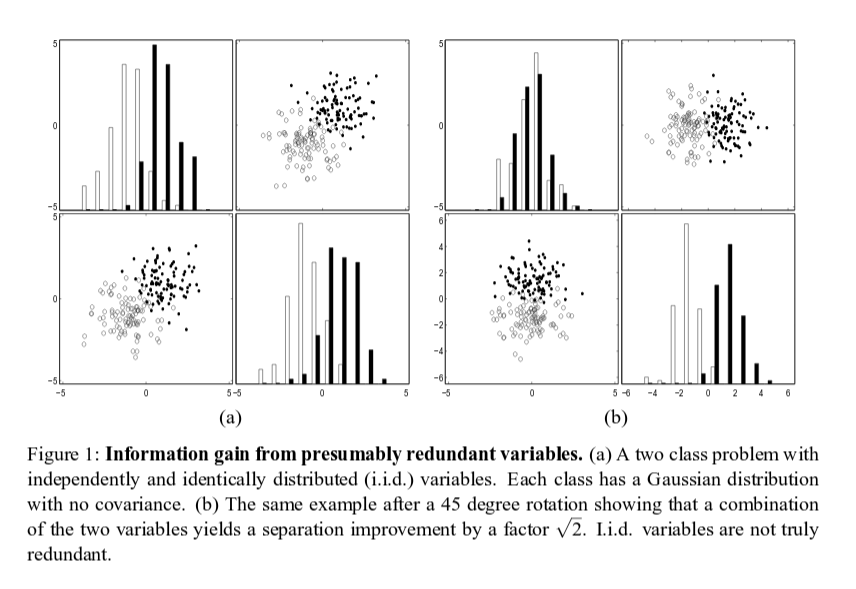
\includegraphics[width=9cm]{figure_man/varsel_ex0.png}
\end{figure}

\begin{center}
\footnotesize{Isabelle Guyon, André Elisseeff (2003). An Introduction to Variable and Feature Selection.  Journal of Machine Learning Research (3) p. 1157-1182.}
\end{center}

\framebreak

\begin{figure}
  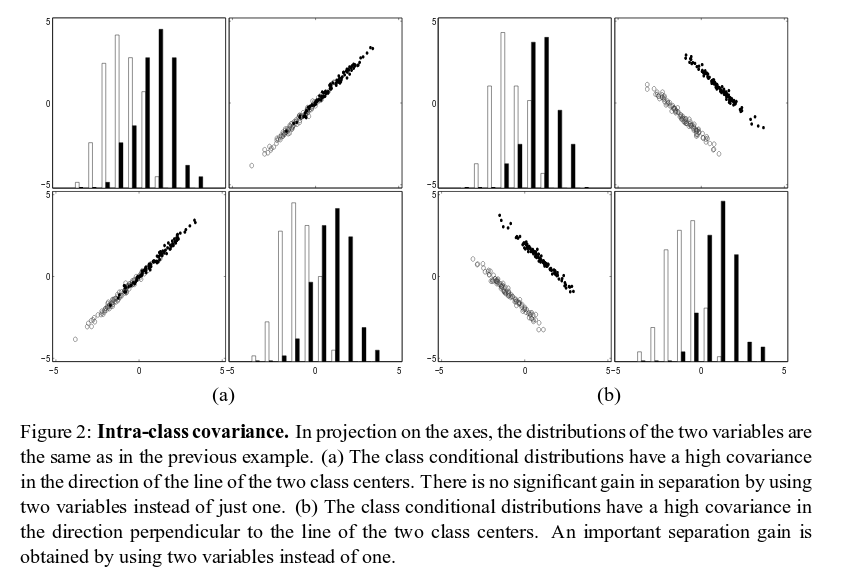
\includegraphics[width=9cm]{figure_man/varsel_ex1.png}
\end{figure}

\begin{center}
\footnotesize{Isabelle Guyon, André Elisseeff (2003). An Introduction to Variable and Feature Selection.  Journal of Machine Learning Research (3) p. 1157-1182.}
\end{center}

\framebreak

\begin{figure}
  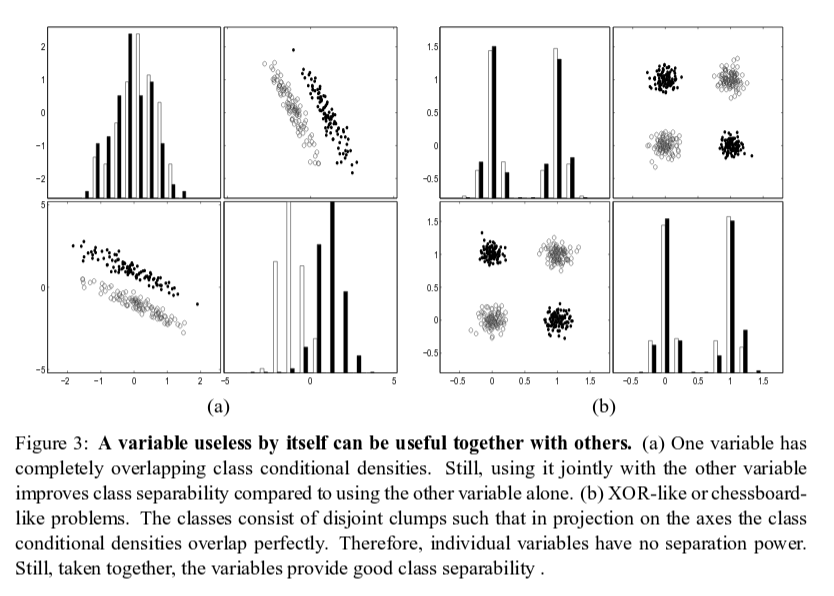
\includegraphics[width=9cm]{figure_man/varsel_ex2.png}
\end{figure}

\begin{center}
\footnotesize{Isabelle Guyon, André Elisseeff (2003). An Introduction to Variable and Feature Selection.  Journal of Machine Learning Research (3) p. 1157-1182.}
\end{center}

\end{vbframe}



\begin{vbframe}{Filter: $\chi^2$-statistic}
\begin{itemize}
  \item Test for independence between the $j$-th feature and the target $y$.
  \item Numeric features or targets need to be discretized.
  \item Hypotheses:

  $H_0: p(x_j = l, y = k) = p(x_j = l)\, p(y = k)$, $\forall j = 1, \dots, k_1$

  \noindent\hspace*{6.55cm} $\forall k = 1, \dots, k_2$

  $H_1: \exists \; j, k: p(x_j = l, y = k) \neq p(x_j = l)\, p(y = k)$
  \item Calculate the $\chi^2$-statistic for each feature-target combination:
    $$ \chi^2 = \sum_{j = 1}^{k_1} \sum_{k=1}^{k_2} (\frac{e_{jk} - \tilde{e}_{jk}}{\tilde{e}_{jk}}) \;\;\;   \stackrel{H_0}{\underset{approx.}{\sim}} \; \chi^2 ((k_1-1)(k_2-1))$$
  where $e_{jk}$ is the observed relative frequency of pair $(j,k)$ and $\tilde{e}_{jk} = \frac{e_{j \cdot} e_{\cdot k}}{n}$ is the expected relative frequency.
  \item The greater $\chi^2$, the more dependent is the feature-target combination, the more relevant is the feature.
\end{itemize}
\end{vbframe}


\begin{vbframe}{Filter: Pearson \& Spearman correlation}
\textbf{Pearson correlation $r(\xj, y)$: }
\begin{itemize}
  \item For numeric features and targets only.
  \item Most sensitive for linear or monotonic relationships.
  \item $ r(\xj, y) = \frac{\sum_{i=1}^n (x^{(i)}_j - \bar{x}_j) (\yi - \bar{y})}{\sqrt{\sum_{i=1}^n (x^{(i)}_j - \bar{x}_j)} \sqrt{(\sum_{i=1}^n \yi - \bar{y})}},\qquad -1 \le r \le 1$
\end{itemize}
\textbf{Spearman correlation $r_{SP}(\xj, y)$:}
\begin{itemize}
  \item For features and targets at least on an ordinal scale.
  \item Equivalent to Pearson correlation computed on the ranks.
  \item Assesses monotonicity of the dependency relationship.
  % \item Calculate the Spearman correlation coefficient between each feature-target combination:
  % $$ r_{SP} = \frac{\sum (rg(\xi) - \bar{rg}_x) (rg(\yi) - \bar{rg}_y)}{\sqrt{\sum (rg(\xi) - \bar{rg}_x)^2 \sum (rg(\yi) - \bar{rg}_y)^2}}$$
  % $-1 \le r_{SP} \le 1$
  % 
  % $r_{SP} > 0$: positive correlation.
  % 
  % $r_{SP} < 0$: negative correlation.
  % 
  % $r_{SP} = 0$: no correlation.
  % \item A higher score indicates a higher relevance of the feature.
\end{itemize}
\lz
Use absolute values $|r(\xj, y)|$ for feature ranking: higher score indicates a higher relevance.

\framebreak

Only \textbf{linear} dependency structure, non-linear (non-monotonic) aspects are not captured by $r$:

\lz

% in rsrc/chunk2_filter_correlation.R created
\begin{figure}
  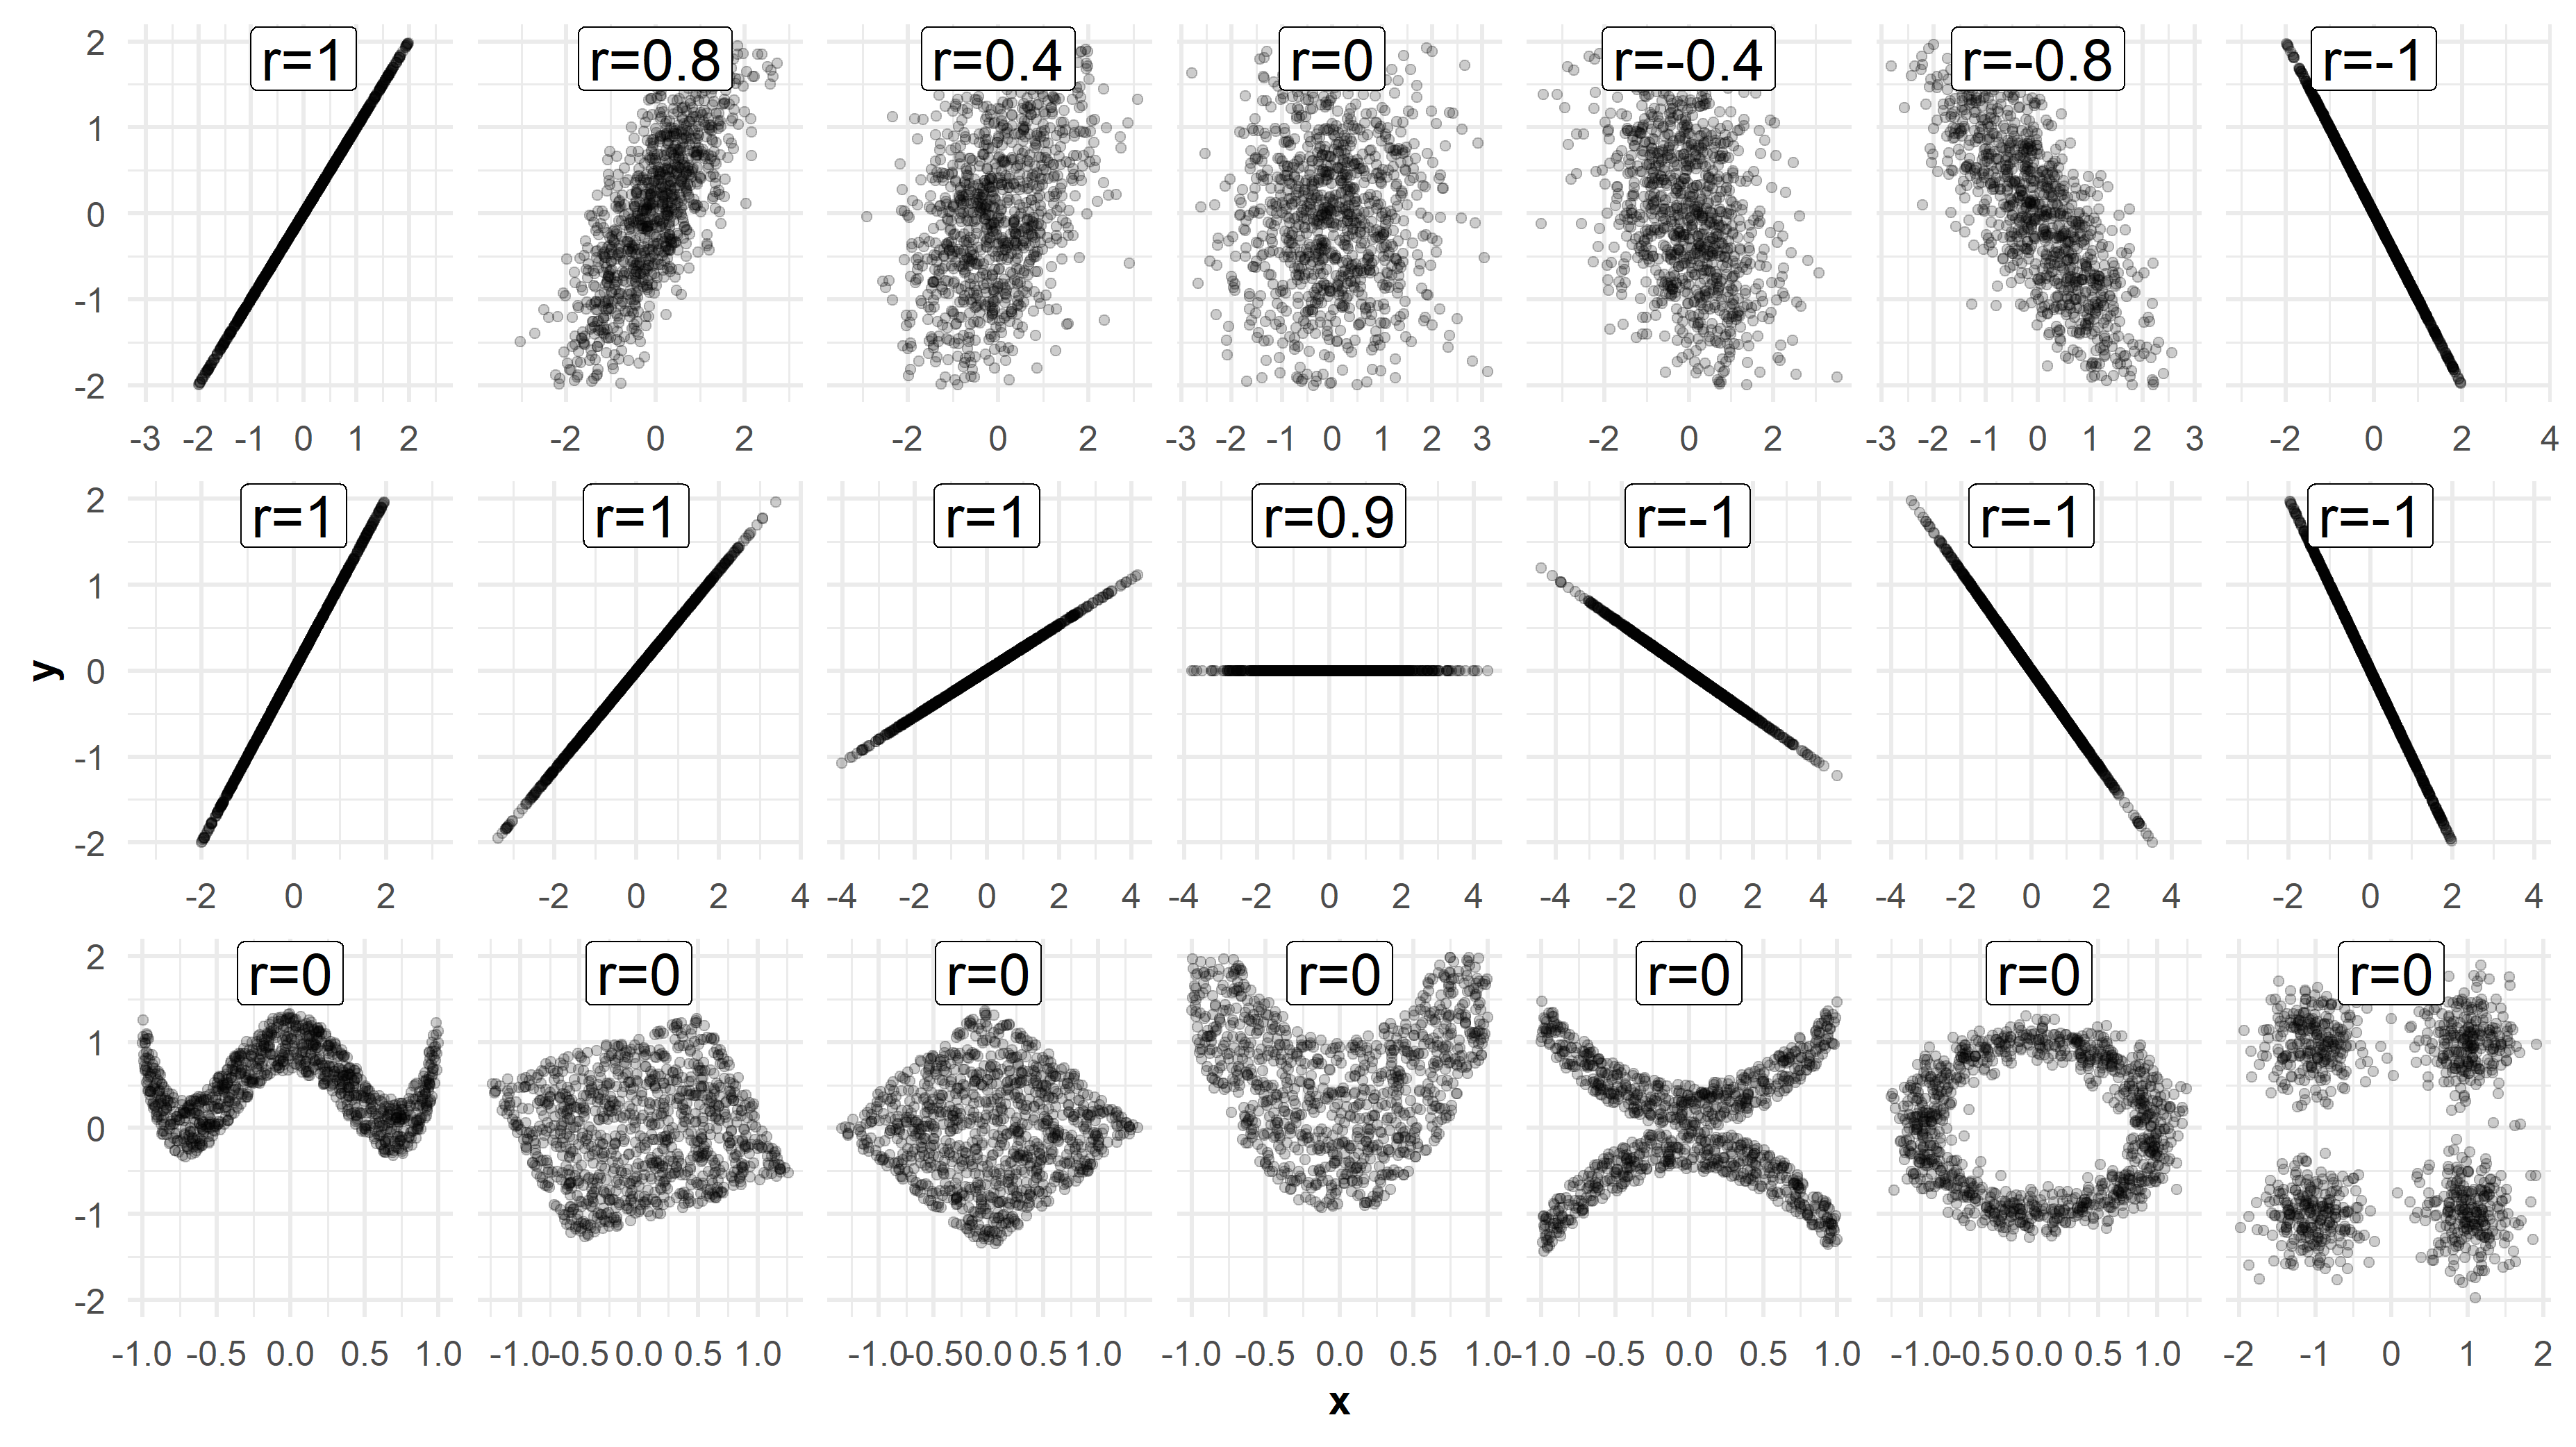
\includegraphics {figure_man/chunk2_filter_correlation.png}
\end{figure}

% \begin{center}
%   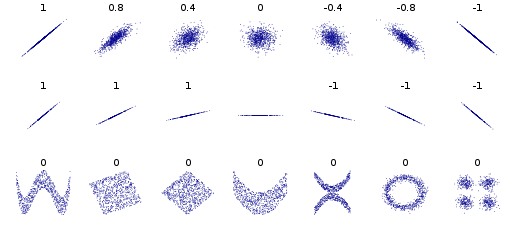
\includegraphics[width=0.9\textwidth]{figure_man/correlation_example.png}
% 
%   \scriptsize{\url{https://en.wikipedia.org/wiki/Pearson\_correlation\_coefficient\#/media/File:Correlation\_examples2.svg}}
% \end{center}
% 
% \begin{vbframe}{Filter: Rank correlation}
% \begin{itemize}
%   \item For features and targets at least on ordinal scale.
%   \item Equivalent to Pearson correlation computed on the ranks.
%   \item Assesses monotonicity of the dependency relationship.
  % \item Calculate the Spearman correlation coefficient between each feature-target combination:
  % $$ r_{SP} = \frac{\sum (rg(\xi) - \bar{rg}_x) (rg(\yi) - \bar{rg}_y)}{\sqrt{\sum (rg(\xi) - \bar{rg}_x)^2 \sum (rg(\yi) - \bar{rg}_y)^2}}$$
  % $-1 \le r_{SP} \le 1$
  % 
  % $r_{SP} > 0$: positive correlation.
  % 
  % $r_{SP} < 0$: negative correlation.
  % 
  % $r_{SP} = 0$: no correlation.
  % \item A higher score indicates higher relevance of the feature.
%   \end{itemize}
% \end{vbframe}
\end{vbframe}

\begin{vbframe}{Filter: Distance correlation}
% sources: 
%Szekely, G.J., Rizzo, M.L., and Bakirov, N.K. (2007), Measuring and Testing Dependence by Correlation of Distances, Annals of Statistics, Vol. 35 No. 6, pp. 2769-2794. 
% http://dx.doi.org/10.1214/009053607000000505
%Szekely, G.J. and Rizzo, M.L. (2009), Brownian Distance Covariance, Annals of Applied Statistics, Vol. 3, No. 4, 1236-1265. 
% http://dx.doi.org/10.1214/09-AOAS312 

$$r_D(\xj, y) = \sqrt{\frac{c_{D}^2(\xj, y)}{\sqrt{c_{D}^2(\xj, \xj) c_{D}^2(y, y)}}}:$$
Normed version of \textbf{distance covariance} $c_{D}(\xj, y) = \frac{1}{n^2}\sum^n_{i=1}\sum^n_{k=1} D^{(ik)}_{\xj} D^{(ik)}_{y}$ for
\begin{itemize}
\item distances of observations: $d\left(x^{(i)}_j, x^{(k)}_j\right)$,
\item mean distances $\bar{d}^{(i\cdot)}_{xj} = \tfrac{1}{n} \sum^n_{k=1} d\left(x^{(i)}_j, x^{(k)}_j\right)$,
\item and centered pairwise distances
$D^{(ik)}_{x} = d\left(x^{(i)}_j, x^{(k)}_j\right) - (\bar{d}^{(i\cdot)}_{xj} + \bar{d}^{(\cdot k)}_{xj} - \bar{d}^{(\cdot \cdot)}_{xj})$
\end{itemize}

\framebreak

Properties:
\begin{itemize}
\item $0 \leq r_D(\xj, y) \leq 1 \quad \forall  j \in \{1, …, p\}$
\item $r_D(\xj, y) = 0$ only if $\xv$ and $y$ are empirically independent (!)
\item $r_D(\xj, y) = 1$ for exact linear dependencies
\item also assesses strength of \textbf{non-monotonic}, \textbf{non-linear}  dependencies
\item very generally applicable since it only requires distance measures on $\Xspace$ and $\Yspace$: can also be used for ranking multivariate features, feature combinations or non-tabular inputs (text, images, audio, etc.)
\item expensive to compute for large data (i.e., use a subsample)
\end{itemize}

\begin{figure}
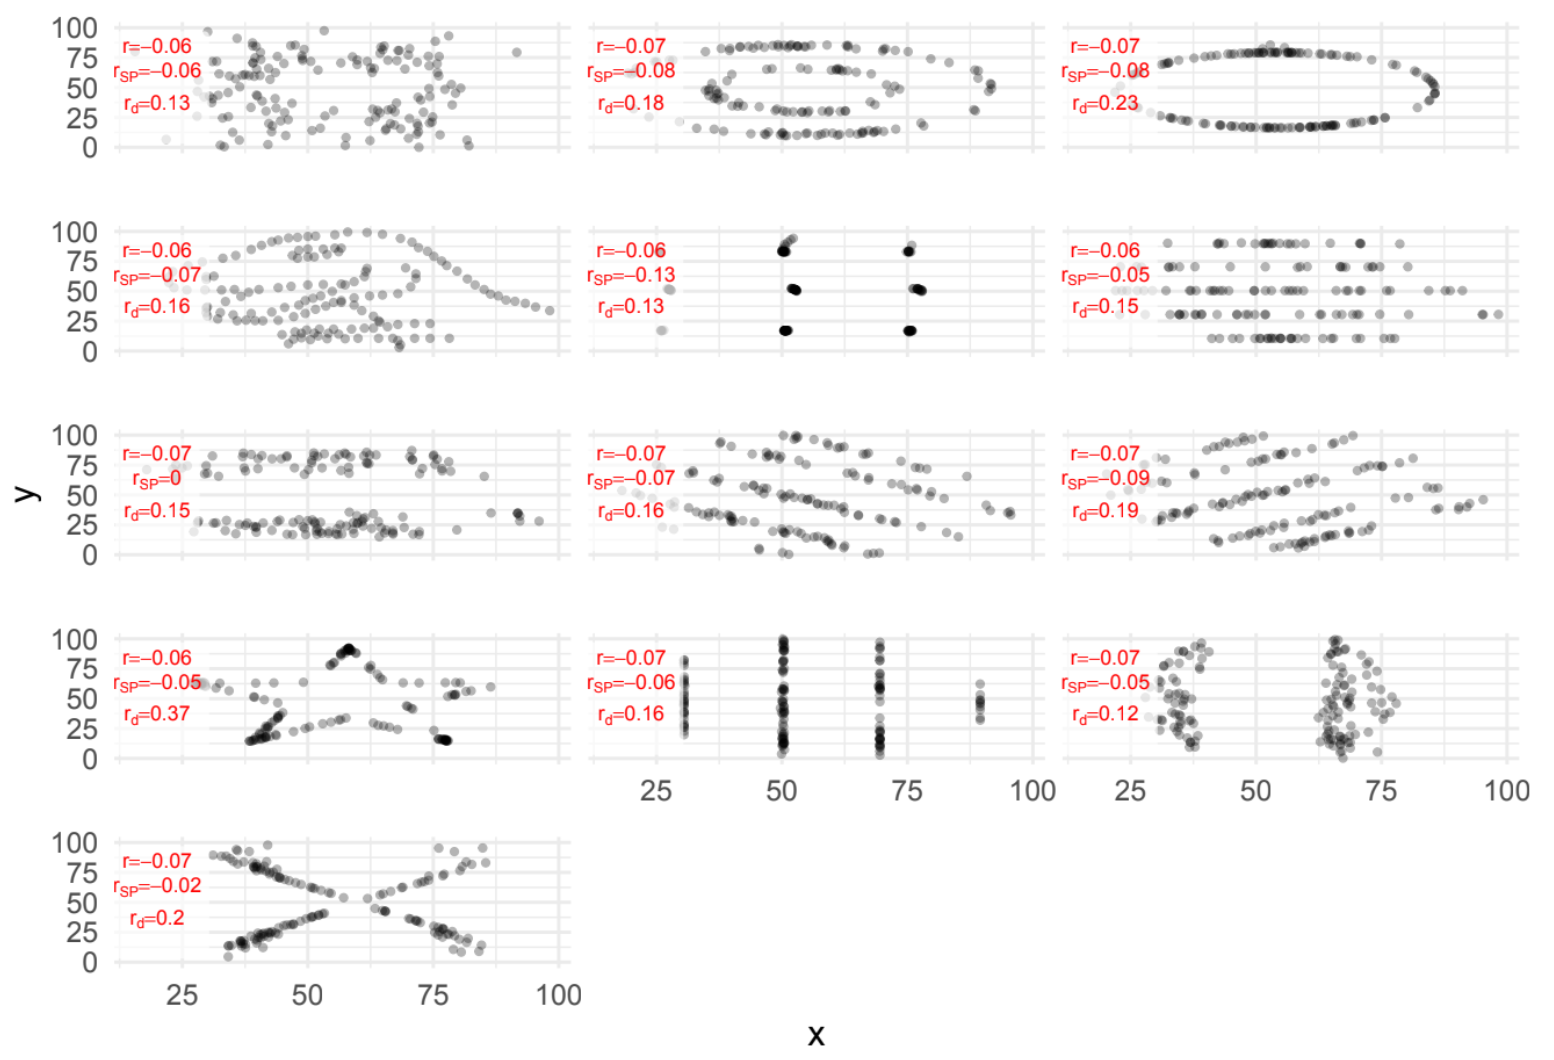
\includegraphics[width = 0.9\textwidth]{figure_man/distance-corre.png}
\end{figure}


\end{vbframe}




\begin{vbframe}{Filter: Welch's \MakeLowercase{t}-test}
\begin{itemize}
  \item For binary classification with numeric features.
  \item Test for unequal means of the $j$-th feature.
  \item For notational purposes let $\Yspace \in \{ 0, 1\}$. Then the subscript $j_0$ refers to the $j$-th feature where $y = 0$ and $j_1$ where $y = 1$.
  \item Hypotheses:

  $H_0$: $\;\;\mu_{j_0} = \mu_{j_1} $ \qquad vs. \qquad $H_1$: $\;\;\mu_{j_0} \neq \mu_{j_1}$
  \item Calculate Welch's t-statistic for every feature $\xj$
  $$ t_j = \frac{\bar{x}_{j_0} - \bar{x}_{j_1}}{\sqrt{(\frac{S^2_{\xjNull}}{n_0} + \frac{S^2_{\xjEins}}{n_1})}}$$
  where $\bar{x}_{j_0}$, $S^2_{\xjNull}$ and $n_0$ are the sample mean, the population variance and the sample size for y = 0, respectively.
  \item A higher t-score indicates higher relevance of the feature.
\end{itemize}
\end{vbframe}


\begin{vbframe}{Filter: F-Test}
\begin{itemize}
  \item For multiclass classification ($g \ge 2$) and numeric features.
  \item Assesses whether the expected values of a feature $\xj$ within the classes of the target differ from each other.
  \item Hypotheses:

  $H_0: \mu_{j_0} = \mu_{j_1} = \dots = \mu_{j_g} \;\;\;\;$ vs. $\;\;\;\;H_1 : \exists \; k,l: \mu_{j_k} \neq \mu_{j_l}$
  \item Calculate the F-statistic for each feature-target combination:
  \begin{align*}
  F &= \frac{\text{between-group variability}}{\text{within-group variability}}\\
  F &= \frac{\sum_{k = 1}^g n_k (\bar{x}_{j_k} - \bar{x_j})^2/(g-1)}{\sum_{k = 1}^g \sum_{i = 1}^{n_k} (x_{j_k}^{(i)} - \bar{x}_{j_k})^2/(n-g)}
  \end{align*}
  where $\bar{x}_{j_k}$ is the sample mean of feature $\xj$ where $y = k$ and $\bar{x_{j}}$ is the overall sample mean of feature $\xj$.
\item A higher F-score indicates higher relevance of the feature.
\end{itemize}
\end{vbframe}

\begin{vbframe}{Filter: Mutual Information}
$$I(X ; Y) = \E_{p(x, y)} \left[ \log \frac{p(X, Y)}{p(X) p(Y)} \right]$$

\begin{itemize}
  \item Each variable $\xj$ is rated according to $I(\xj;y)$, this is sometimes called information gain.
  \item MI is a measure of the amount of "dependence" between variables. It is zero if and only if the variables are independent.
  \item On the other hand, if one of the variables is a deterministic function of the other, the mutual information is maximal.
 \item Unlike (Pearson) correlation, mutual information is not limited to real-valued random variables.
   \item Mutual information can be seen as a more general measure of dependence between variables than correlation.
\end{itemize}
\end{vbframe}

\begin{vbframe}{Filter}
\begin{blocki}{How to combine a filter with a model:}
  \item Calculate filter-values.
  \item Sort features by value.
%  \item Choose $\tilde{p}$ best features.
  \item Train model on $\tilde{p}$ best features.
\end{blocki}

\lz

\begin{blocki}{How to choose $\tilde{p}$:}
  \item It can be prescribed by the application.
  \item Eyeball estimation: Read from filter plots (i.e., Scree plots).
  \item Use resampling.
\end{blocki}

\framebreak

\begin{blocki}{Advantages:}
  \item Easy to calculate.
  \item Typically scales well with the number of features $p$.
  \item Mostly interpretable intuitively.
  \item Combination with every model possible.
\end{blocki}

\begin{blocki}{Disadvantages:}
  \item Often univariate (not always) ignores multivariate dependencies.
  \item Redundant features will have similar weights.
  \item Ignores the learning algorithm.
\end{blocki}
\end{vbframe}

\begin{vbframe}{Minimum Redundancy Maximum Relevancy}
\begin{itemize}
  \item Most filter type methods select top-ranked features based on a certain filter method ($\chi^2$, rank-correlation, t-test,...) without considering relationships among the features.
  \item Problems:
  \begin{itemize}
  \item Features may be correlated and hence, may cause redundancy.
  \item Selected features cover narrow regions in space.
  \end{itemize}
  \item Goal: In addition to maximum relevancy of the features we want the features to be maximally dissimilar to each other (minimum redundancy).
  \item Features can be either continuous or categorical.
\end{itemize}
\end{vbframe}

\begin{vbframe}{\MakeLowercase{M}RMR: Criterion functions}
\begin{itemize}
\item Let $S \subset \{1, \dots, p \}$ be a subset of features we want to find.
\item Minimize redundancy

 $$\min \text{Red}(S), \;\;\;\; \text{Red}(S) = \frac{1}{|S|^2} \sum_{j, l \in S} I_{xx}(\xj, \xl)$$

\item Maximize relevancy

 $$\max \text{Rel}(S), \;\;\;\; \text{Rel}(S) = \frac{1}{|S|} \sum_{j \in S} I_{xy}(\xj, \ydat)$$

\item $I_{xx}$ measures the strength of the dependency between two features.
\item $I_{xy}$ measures the strength of the dependency between a feature and the target.
\end{itemize}

\framebreak

\begin{itemize}

\lz

\item Examples for $I_{xx}$:
  \begin{itemize}
  \item Two discrete features: mutual information $I(\xj, \xl)$
  \item Two numeric features: correlation $|r(\xj, \xl)|$
  \end{itemize}

\lz

\item Examples for $I_{xy}$:
  \begin{itemize}
  \item Discrete feature, discrete target: mutual information $I(\xj, \ydat)$
  \item Continuous feature, discrete target: F-statistic $F(\xj, \ydat)$
  \end{itemize}
\end{itemize}


\framebreak

\begin{itemize}
\item The mRMR feature set is obtained by optimizing the relevancy and the redundancy criterion simultaneously.
\item This requires combining the criteria into a single objective function:
$$\Psi(S) = (\text{Rel}(S) - \text{Red}(S)) \;\;\;\; \text{ or } \;\;\;\; \Psi(S) = (\text{Rel}(S)/\text{Red}(S))$$

%\item Exact solution requires $\mathcal{O}(|\Xspace|^{|S|})$ searches, where $|\Xspace|$ is the number of features in the whole feature set and $|S|$ is the number of features selected.
\end{itemize}
In practice, incremental search methods are used to find near-optimal feature sets defined by $\Psi$:
\begin{itemize}
\item Suppose we already have a feature set with $m-1$ features $S_{m-1}$.
\item Next, we select the $m$-th feature from the set $\bar{S}_{m-1}$ by selecting the feature that maximizes:
$$\max_{j \, \in \, \bar{S}_{m-1}} \Biggl[ I_{xy} (\xj, \ydat) - \frac{1}{|S_{m-1}|} \sum_{l \, \in \, S_{m-1}} I_{xx}(\xj, \xl)  \Biggr]$$
\item The complexity of this incremental algorithm is $\mathcal{O}(|p| \cdot| S|)$.
\end{itemize}
\end{vbframe}

\begin{vbframe}{\MakeLowercase{m}RMR: Algorithm}

\begin{algorithm}[H]
\footnotesize
  \begin{algorithmic}[1]
    \State Set $S = \emptyset$, $R = \{ 1, \dots, p \}$
    \State Find the feature with maximum relevancy:
    $$j^* := \argmax_{j} I_{xy} (\xj, \ydat)$$
    \State Set $S = \{ j^* \}$ and update $R \leftarrow R \setminus \{j^* \}$
    \Repeat
      \State Find feature $\xj$ that maximizes:
      $$\max_{j \, \in \, R} \Biggl[ I_{xy} (\xj, \ydat) - \frac{1}{|S|} \sum_{l \, \in \, S} I_{xx}(\xj, \xl)  \Biggr]$$
      \State Update $S \leftarrow S \cup \{j^* \}$ and $R \leftarrow R \setminus \{ j^* \}$
    \Until{Expected number of features have been obtained or some other constraints are satisfied.}
    \caption{mRMR algorithm}
  \end{algorithmic}
\end{algorithm}
\end{vbframe}


% \begin{vbframe}{Filter: Practical example}
% <<echo=TRUE>>=
% # Calculate the information gain as filter value
% fv = generateFilterValuesData(iris.task, method = "information.gain")
%
% # We can also pass multiple filter methods at once:
% fv2 = generateFilterValuesData(iris.task,
%   method = c("information.gain", "chi.squared"))
%
% # fv2 is a FilterValues object and fv2$data holds a data frame
% # with the importance values for all features
% fv2$data
% @
%
% <<>>=
% plotFilterValues(fv2) + ggtitle("Filters for the 4 features of iris dataset")
% @
%
%
% \framebreak
%
% <<size="tiny", echo=TRUE>>=
% ## Keep the 2 most important features
% filtered.task = filterFeatures(iris.task, method = "information.gain", abs = 2L)
%
% ## Keep the 25% most important features
% filtered.task = filterFeatures(iris.task, fval = fv, perc = 0.25)
%
% ## Keep all features with importance greater than 0.5
% filtered.task = filterFeatures(iris.task, fval = fv, threshold = 0.5)
% filtered.task
% @
%
% \framebreak

% \begin{itemize}
%   \item Filter methods are often part of the data preprocessing process, wherein a subsequent step, a learning method is applied.
%   \item In practice we want to automate this, so the feature selection can be part of the validation method of our choice:
% \end{itemize}
% 
% <<size="tiny", echo=TRUE>>=
% lrn = makeFilterWrapper(learner = "classif.kknn",
%   fw.method = "anova.test", fw.abs = 2L)
% ps = makeParamSet(
%   makeDiscreteParam("fw.abs", values = 1:4)
% )
% ctrl = makeTuneControlGrid()
% rdesc = makeResampleDesc("CV", iters = 10L)
% 
% res = tuneParams(lrn, task = iris.task, resampling = rdesc, par.set = ps,
%   control = ctrl)
% res$opt.path
% @
% \end{vbframe}

\endlecture
\end{document}

